\newcommand{\FigAbstractSyntax}{
  \begin{figure}
    \begin{grammar}
      \nt{\expr}{\Expr} & & \grmk{Expressions} \\
      \noalt & \var & \grmk{Variable reference} \\
      & \ttsexp{\text{\tt array}}{\ttparens{\sequence{\nat}} \; \sequence{\atom}}
      & \grmk{Array, containing atoms} \\
      & \ttsexp{\text{\tt array}}{\ttparens{\sequence{\nat}} \; \type}
      & \grmk{Empty array, with its atom type} \\
      & \ttsexp{\text{\tt frame}}{\ttparens{\sequence{\nat}} \; \sequence{\expr}}
      & \grmk{Frame, containing array cells} \\
      & \ttsexp{\text{\tt frame}}{\ttparens{\sequence{\nat}} \; \sequence{\expr}}
      & \grmk{Empty frame, with its cell type} \\
      & \ttsexp{\expr_f}{\sequence{\expr_a}}
      & \grmk{Term application} \\
      & \ttsexp{\text{\tt t-app}}{\expr \; \sequence{\type}}
      & \grmk{Type application} \\
      & \ttsexp{\text{\tt i-app}}{\expr \; \sequence{\idx}}
      & \grmk{Index application} \\
      & \ttsexp{\text{\tt unbox}}{\ttparens{\sequence{\var_i} \; \var_e \; \expr_s} \; \expr_b}
      & \grmk{Let-binding box contents} \\
      \nt{\val}{\Val} & \var \gramalt \ttsexp{\text{\tt array}}{\ttparens{\sequence{\nat}} \; \sequence{\atval}} & \grmk{Values} \\
      \nt{\atom}{\Atom} & & \grmk{Atoms} \\
      \noalt & \baseval & \grmk{Base value} \\
      & \primop & \grmk{Primitive operator} \\
      & \lam{\sequence{\notevar{\var}{\type}}}{\expr} & \grmk{Term abstraction} \\
      & \tlam{\sequence{\notevar{\var}{\kind}}}{\val} & \grmk{Type abstraction} \\
      & \ilam{\sequence{\notevar{\var}{\sort}}}{\val} & \grmk{Index abstraction} \\
      & \dsum{\sequence{\idx}}{\expr}{\type} & \grmk{Boxed array} \\
      \nt{\atval}{\Atval} &
      \baseval \gramalt \primop \gramalt \lam{\sequence{\notevar{\var}{\type}}}{\expr}
      \gramalt \tlam{\sequence{\notevar{\var}{\kind}}}{\val}
      & \grmk{Atomic values} \\
      % \noalt & \baseval & \grmk{Base value} \\
      % & \primop & \grmk{Primitive operator} \\
      % & \lam{\sequence{\notevar{\var}{\type}}}{\expr} & \\
      & \ilam{\sequence{\notevar{\var}{\sort}}}{\val} \gramalt \dsum{\sequence{\idx}}{\val}{\type}  & \\
      % & \ilam{\sequence{\notevar{\var}{\sort}}}{\val} & \\
      % & \dsum{\sequence{\idx}}{\val}{\type} & \\
      \nt{\type}{\Type} & & \grmk{Types} \\
      \noalt & \var & \grmk{Type variable} \\
      & \basetype & \grmk{Base type} \\
      & \typearray{\type}{\idx} & \grmk{Array} \\
      & \typefun{\sequence{\type}}{\type'} & \grmk{Function} \\
      & \typeuniv{\sequence{\notevar{\var}{\kind}}}{\type} & \grmk{Universal} \\
      & \typedprod{\sequence{\notevar{\var}{\sort}}}{\type} & \grmk{Dependent product} \\
      & \typedsum{\sequence{\notevar{\var}{\sort}}}{\type} & \grmk{Dependent sum} \\
      \nt{\kind}{\Kind} & \kindarray \gramalt \kindatom & \grmk{Kinds} \\
      \nt{\idx}{\Idx} & & \grmk{Type indices} \\
      \noalt & \var & \grmk{Type variable} \\
      & \nat & \grmk{Single dimension} \\
      & \idxshape{\sequence{\idx}} & \grmk{Sequence of dimensions)} \\
      & \idxadd{\sequence{\idx}} & \grmk{Adding dimensions} \\
      & \idxappend{\sequence{\idx}} & \grmk{Appending shapes} \\
      \nt{\sort}{\Sort} & \sortshp \gramalt \sortdim & \grmk{Index sorts} \\
      \nt{\primop}{\Primop} &
      \text{\tt +} \gramalt \text{\tt -} \gramalt \text{\tt *} \gramalt \text{\tt /} \gramalt
      \text{\tt append} \gramalt \text{\tt reduce} \gramalt \text{\tt iota} \gramalt \text{\tt ...}
      & \grmk{Primitive operators} \\
      \nt{\func}{\Func} & \primop \gramalt \expr & \grmk{Functions} \\
      \nt{\term}{\Term} & \atom \gramalt \lam{\sequence{\notevar{\var}{\type}}}{\expr} & \grmk{Terms} \\
    \end{grammar}
    \caption{Core Remora grammar}
    \label{fig:AbstractSyntax}
  \end{figure}
}


\newcommand{\FigSortingRules}{
  \begin{figure}
    \fbox{$\sortof{\sEnv}{\idx}{\sort}$}
    \begin{mathpar}
      \infr[S-Nat]
      {\nat \in \mathbb{N}}
      {\sortof
        {\sEnv}
        {\nat}
        {\sortdim}}
      \and
      \infr[S-Var]
      {\parens{\hassort{\var}{\sort}} \in \sEnv}
      {\sortof
        {\sEnv}
        {\var}
        {\sort}}
      \and
      \infr[S-Shape]
      {\seqpremise{j}
        {\sortof
          {\sEnv}
          {\idx_j}
          {\sortdim}}}
      {\sortof
        {\sEnv}
        {\idxshape{\sequence{\idx}}}
        {\sortshp}}
      \and
      \infr[S-Plus]
      {\seqpremise{j}
        {\sortof
          {\sEnv}
          {\idx_j}
          {\sortdim}}}
      {\sortof
        {\sEnv}
        {\idxadd{\sequence{\idx}}}
        {\sortdim}}
      \and
      \infr[S-Append]
      {\seqpremise{j}
        {\sortof
          {\sEnv}
          {\idx_j}
          {\sortshp}}}
      {\sortof
        {\sEnv}
        {\idxappend{\sequence{\idx}}}
        {\sortshp}}
    \end{mathpar}
    \caption{Sorting rules}
    \label{fig:SortingRules}
  \end{figure}
}

\newcommand{\FigKindingRules}{
  \begin{figure}
    \fbox{$\kindof{\sEnv}{\kEnv}{\type}{\kind}$}
    \begin{mathpar}
      \infr[K-Var]
      {\parens{\haskind{\var}{\kind}} \in \kEnv}
      {\kindof{\sEnv}{\kEnv}{\var}{\kind}}
      \and
      \infr[K-Base]
      {\quad}
      {\kindof{\sEnv}{\kEnv}{\basetype}{\kindatom}}
      \and
      \infr[K-Fun]
      {\seqpremise{j}{\kindof{\sEnv}{\kEnv}{\type_j}{\kindarray}}
        \\\\
        \kindof{\sEnv}{\kEnv}{\type'}{\kindarray}}
      {\kindof{\sEnv}{\kEnv}{\typefun{\sequence{\type}}{\type'}}{\kindatom}}
      \and
      \infr[K-Univ]
      {\kindof{\sEnv}{\kEnv, \sequence{\haskind{\var}{\kind}}}{\type}{\kindarray}}
      {\kindof{\sEnv}{\kEnv}{\typeuniv{\sequence{\notevar{\var}{\kind}}}{\type}}{\kindatom}}
      \and
      \infr[K-Pi]
      {\kindof{\sEnv, \sequence{\hassort{\var}{\sort}}}{\kEnv}{\type}{\kindarray}}
      {\kindof{\sEnv}{\kEnv}{\typedprod{\sequence{\notevar{\var}{\sort}}}{\type}}{\kindatom}}
      \and
      \infr[K-Sigma]
      {\kindof{\sEnv, \sequence{\hassort{\var}{\sort}}}{\kEnv}{\type}{\kindarray}}
      {\kindof{\sEnv}{\kEnv}{\typedsum{\sequence{\notevar{\var}{\sort}}}{\type}}{\kindatom}}
      \and
      \infr[K-Array]
      {\sortof{\sEnv}{\idx}{\sortshp}
       \\
       \kindof{\sEnv}{\kEnv}{\type}{\kindatom}}
      {\kindof{\sEnv}{\kEnv}{\typearray{\type}{\idx}}{\kindarray}}
      \rulename{K-Array}
    \end{mathpar}
    \caption{Kinding rules}
    \label{fig:KindingRules}
  \end{figure}
}

\newcommand{\FigTypingRules}{
  \begin{figure}
    \fbox{$\typeof{\sEnv}{\kEnv}{\tEnv}{\term}{\type}$}
    \begin{mathpar}
      \infr[T-Op]
      {\ }
      {\typeof{\sEnv}{\kEnv}{\tEnv}{\primop}{\Sigref{\primop}}}
      \and
      \infr[T-Var]
      {\parens{\hastype{\var}{\type}} \in \tEnv}
      {\typeof{\sEnv}{\kEnv}{\tEnv}{\var}{\type}}
      \and
      \infr[T-Eqv]
      {\typeof{\sEnv}{\kEnv}{\tEnv}{\term}{\type'}\\
       \teqv{\type}{\type'}}
      {\typeof{\sEnv}{\kEnv}{\tEnv}{\term}{\type}}
      \and
      \infr[T-Array]
      {\seqpremise{j}{\typeof
          {\sEnv}{\kEnv}{\tEnv}
          {\atom_j}{\type}}
        \\\\
        \kindof{\sEnv}{\kEnv}{\type}{\kindatom}
        \\\\
        \mathit{Length}\llb \sequence{\atom} \rrb = \prod{\sequence{\nat}}}
      {\parbox{0.35\textwidth}
        {\({\sEnv};{\kEnv};{\tEnv}\vdash\)
          \({\arrlit{\sequence{\atom}}{\sequence{\nat}}}\)\\
          \(:{\typearray{\type}{\idxshape{\sequence{\nat}}}}\)}}
      \and
      \infr[T-0A]
      {\kindof{\sEnv}{\kEnv}{\type}{\kindatom}
        \\\\
        0 \in \sequence{\nat}}
      {\parbox{0.30\textwidth}
        {\({\sEnv};{\kEnv};{\tEnv}\vdash\)
          \({\emptyarrlit{\type}{\sequence{\nat}}}\)\\
          \(:{\typearray{\type}{\idxshape{\sequence{\nat}}}}\)}}
      \and
      \infr[T-Frame]
      {\seqpremise{j}{\typeof
          {\sEnv}{\kEnv}{\tEnv}
          {\expr_j}{\typearray{\type}{\idx}}}
        \\\\
        \kindof{\sEnv}{\kEnv}{\typearray{\type}{\idx}}{\kindarray}
        \\\\
        \mathit{Length}\llb \sequence{\expr} \rrb = \prod{\sequence{\nat}}}
      {\parbox{0.35\textwidth}
        {\({\sEnv};{\kEnv};{\tEnv}\vdash\)
          \({\frm{\sequence{\expr}}{\sequence{\nat}}}\)\\
          \(:{\typearray{\type}{\idxappend{\idxshape{\sequence{\nat}} \; \idx}}}\)}}
      \and
      \infr[T-0F]
      {\kindof{\sEnv}{\kEnv}{\type}{\kindatom}
        \\\\
        \sortof{\sEnv}{\idx}{\sortshp}
        \\
        0 \in \sequence{\nat}}
      {\parbox{0.38\textwidth}
        {\({\sEnv};{\kEnv};{\tEnv}\vdash\)
          \({\emptyfrm{\typearray{\type}{\idx}}{\sequence{\nat}}}\)\\
          \(:{\typearray{\type}{\idxappend{\idxshape{\sequence{\nat}} \; \idx}}}\)}}
      \and
      \infr[T-Lam]
      {\typeof
        {\sEnv}{\kEnv}{\tEnv, \sequence{\hastype{\var}{\type}}}
        {\expr}
        {\type'}
        \\\\
        \seqpremise{j}{\kindof{\sEnv}{\kEnv}{\type}{\kindarray}}}
      {\parbox{0.35\textwidth}
        {\({\sEnv};{\kEnv};{\tEnv}\vdash\)
          \({\lam{\sequence{\notevar{\var}{\type}}}{\expr}}\)\\
          \(:{\typefun{\sequence{\type}}{\type'}}\)}}
      \and
      \infr[T-TLam]
      {\typeof
        {\sEnv}{\kEnv, \sequence{\haskind{\var}{\kind}}}{\tEnv}
        {\val}
        {\type}}
      {\parbox{0.30\textwidth}
        {\({\sEnv};{\kEnv};{\tEnv}\vdash\)
          \({\tlam{\sequence{\notevar{\var}{\kind}}}{\val}}\)\\
          \(:{\typeuniv{\sequence{\notevar{\var}{\kind}}}{\type}}\)}}
      \and
      \infr[T-ILam]
      {\typeof
        {\sEnv, \sequence{\haskind{\var}{\sort}}}{\kEnv}{\tEnv}
        {\val}
        {\type}}
      {\parbox{0.30\textwidth}
        {\({\sEnv};{\kEnv};{\tEnv}\vdash\)
          \({\ilam{\sequence{\notevar{\var}{\sort}}}{\val}}\)\\
          \(:{\typedprod{\sequence{\notevar{\var}{\sort}}}{\type}}\)}}
      \and
      \infr[T-Box]
      {\seqpremise{j}{\sortof{\sEnv}{\idx}{\sort}}
        \\\\
        \kindof{\sEnv}{\kEnv}
        {\typedsum{\sequence{\notevar{\var}{\sort}}}{\type}}
        {\kindatom}
        \\\\
        \typeof
        {\sEnv}{\kEnv}{\tEnv}
        {\expr}
        {\seqsubst{\type}{\var}{\idx}}}
      {\parbox{0.45\textwidth}
        {\({\sEnv};{\kEnv};{\tEnv}\vdash\)
          \({\dsum
            {\sequence{\idx}}
            {\expr}
            {\typedsum{\sequence{\notevar{\var}{\sort}}}{\type}}}\)\\
          \(:{\typedsum{\sequence{\notevar{\var}{\sort}}}{\type}}\)}}
      \and
      \infr[T-TApp]
      {\typeof
        {\sEnv}{\kEnv}{\tEnv}
        {\expr}
        {\typearray{\typeuniv{\sequence{\notevar{\var}{\kind}}}{\typearray{\type_u}{\idx_u}}}{\idx_f}}
        \\
        \seqpremise{j}{\kindof{\sEnv}{\kEnv}{\type_j}{\kind_j}}}
      {\typeof
        {\sEnv}{\kEnv}{\tEnv}
        {\tapp{\expr}{\sequence{\type}}}
        {\typearray{\seqsubst{\type_u}{\var}{\type}}{\idxappend{\idx_f\;\idx_u}}}}
      \and
      \infr[T-IApp]
      {\typeof
        {\sEnv}{\kEnv}{\tEnv}
        {\expr}
        {\typearray{\typedprod{\sequence{\notevar{\var}{\sort}}}{\typearray{\type_p}{\idx_p}}}{\idx_f}}
        \\
        \seqpremise{j}{\sortof{\sEnv}{\idx_j}{\sort_j}}}
      {\typeof
        {\sEnv}{\kEnv}{\tEnv}
        {\iapp{\expr}{\sequence{\idx}}}
        {\typearray
          {\seqsubst{\type_p}{\var}{\idx}}
          {\idxappend{\idx_f\;\seqsubst{\idx_p}{\var}{\idx}}}}}
      \and
      \infr[T-Unbox]
      {\typeof
        {\sEnv}{\kEnv}{\tEnv}
        {\expr_s}
        {\typearray{\typedsum{\sequence{\notevar{\var_i'}{\sort}}}{\type_s}}
          {\idx_s}}
        \\
        \typeof
        {\sEnv,\sequence{\hassort{\var_i}{\sort}}}
        {\kEnv}
        {\tEnv,\hastype{\var_e}{\seqsubst{\type_s}{\var_i'}{\var_i}}}
        {\expr_b}
        {\typearray{\type_b}{\idx_b}}
        \\
        \kindof{\sEnv}{\kEnv}{\typearray{\type_b}{\idx_b}}{\kindarray}}
      {\typeof
        {\sEnv}{\kEnv}{\tEnv}
        {\dproj{\sequence{\var_i}}{\var_e}{\expr_s}{\expr_b}}
        {\typearray{\type_b}{\idxappend{\idx_s \; \idx_b}}}}
      \rulename{T-Unbox}
      \and
      \infr[T-App]
      {\typeof
        {\sEnv}{\kEnv}{\tEnv}
        {\expr_f}
        {\typearray
          {\typefun
            {\sequence{\typearray{\type}{\idx}}}
            {\typearray{\type'}{\idx'}}}
          {\idx_f}}
        \\
        \sequence{\typeof
          {\sEnv}{\kEnv}{\tEnv}
          {{\expr_a}}
          {\typearray{\type}{\idxappend{{\idx_a} \; {\idx}}}}}
        \\
        \idx_p = \displaystyle\bigsqcup\left\{ \idx_f \; \sequence{\idx_a} \right\}}
      {\typeof
        {\sEnv}{\kEnv}{\tEnv}
        {\app{\expr_f}{\sequence{\expr_a}}}
        {\typearray{\type'}{\idxappend{\idx_p \; \idx'}}}}
    \end{mathpar}
    \caption{Typing rules}
    \label{fig:TypingRules}
  \end{figure}
}


\newcommand{\FigTypeEqv}{
 \begin{figure}
   \fbox{$\teqv{\type}{\type'}$}
   \begin{mathpar}
     \infr[TEqv-Refl]
     {\ }
     {\teqv{\type}{\type}}
     \and
     \infr[TEqv-Array]
     {\teqv{\type}{\type'}
       \\
       \ieqv{\idx}{\idx'}
     }
     {\teqv
       {\typearray{\type}{\idx}}
       {\typearray{\type'}{\idx'}}}
     \and
     \infr[TEqv-Fn]
     {\seqpremise{j}{\teqv
         {{\type_i}_j}
         {{\type_i'}_j}}
       \\
       \teqv
       {\type_o}
       {\type_o'}}
     {\teqv
       {\typefun{\sequence{\type_i}}{\type_o}}
       {\typefun{\sequence{\type_i'}}{\type_o'}}}
     \and
     \infr[TEqv-Univ]
     {\teqv
       {\seqsubst{\type}{\var}{\var_f}}
       {\seqsubst{\type'}{\var'}{\var_f}}
       \fresh{\sequence{\var_f}}}
     {\teqv
       {\typeuniv{\sequence{\notevar{\var}{\kind}}}{\type}}
       {\typeuniv{\sequence{\notevar{\var'}{\kind}}}{\type'}}}
     \and
     \infr[TEqv-Pi]
     {\teqv
       {\seqsubst{\type}{\var}{\var_f}}
       {\seqsubst{\type'}{\var'}{\var_f}}
       \fresh{\sequence{\var_f}}}
     {\teqv
       {\typedprod{\sequence{\notevar{\var}{\sort}}}{\type}}
       {\typedprod{\sequence{\notevar{\var'}{\sort}}}{\type'}}}
     \and
     \infr[TEqv-Sigma]
     {\teqv
       {\seqsubst{\type}{\var}{\var_f}}
       {\seqsubst{\type'}{\var'}{\var_f}}
       \fresh{\sequence{\var_f}}}
     {\teqv
       {\typedsum{\sequence{\notevar{\var}{\sort}}}{\type}}
       {\typedsum{\sequence{\notevar{\var'}{\sort}}}{\type'}}}
   \end{mathpar}
   \caption{Type equivalence}
   \label{fig:TypeEqv}
 \end{figure}
}

\newcommand{\FigOverlapAxiom}{
  \begin{figure}
    \begin{center}
      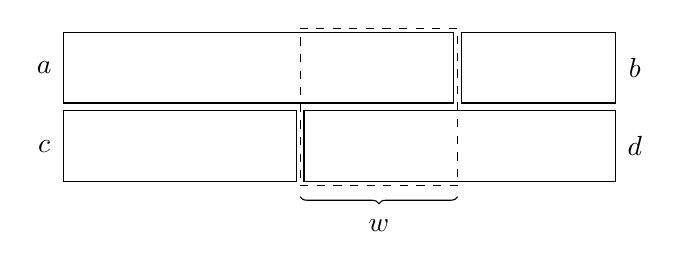
\begin{tikzpicture}
        % a ++ b
        \path (-5.25, 1.5) node (aEdit) {$a$};
        \draw (-5, 1.05) -- (-0.05, 1.05) -- (-0.05, 1.95) -- (-5, 1.95) -- cycle;
        \path (2.25, 1.5) node (bEdit) {$b$};
        \draw (0.05, 1.05) -- (2, 1.05) -- (2, 1.95) -- (0.05, 1.95) -- cycle;
        % c ++ d
        \path (-5.25, 0.5) node (cEdit) {$c$};
        \draw (-5, 0.05) -- (-2.05, 0.05) -- (-2.05, 0.95) -- (-5, 0.95) -- cycle;
        \path (2.25, 0.5) node (dEdit) {$d$};
        \draw (-1.95, 0.05) -- (2, 0.05) -- (2, 0.95) -- (-1.95, 0.95) -- cycle;
        % w
        \path (-1, -0.5) node (wEdit) {$w$};
        \draw [decorate,decoration={brace},xshift=0pt,yshift=-4pt] (0, 0) -- (-2, 0);
        \draw [dashed] (-2, 0) -- (0, 0) -- (0, 2) -- (-2, 2) -- cycle;
      \end{tikzpicture}
    \end{center}
    \caption{Overlap axiom, visualized: $w$ is the overlapping portion of $a$ and $d$.}
    \label{fig:OverlapAxiom}
  \end{figure}
}

\newcommand{\FigListMetafns}{
  \begin{figure}
    \[\mathit{Split}_n\llb \ttparens{a_1, \dots, a_m} \rrb =
    \ttparens{\ttparens{a_1, \dots, a_n}, \ttparens{a_{n+1}, \dots, a_{2n}}, \dots, \ttparens{a_{m-n+1}, \dots, a_m}}\]
    \[\mathit{Rep}_n \llb \ttparens{ a_1, \dots, a_m} \rrb =
    \ttparens{a_{1,1}, \dots, a_{1,n}, \dots, a_{m,1}, \dots, a_{m,n}}
    \quad \text{where } a_{i,j}=a_i\]
    \[\mathit{Concat} \llb \ttparens{\ttparens{a_{1,1}, \dots, a_{1,n}}, \dots, \ttparens{a_{m,1}, \dots, a_{m,n}}} \rrb =
    \ttparens{a_{1, 1}, \dots, a_{1, n}, \dots, a_{m, 1}, \dots, a_{m, n}}\]
    \[\mathit{Transpose}\ttparens{\ttparens{a_{1,1}, \dots, a_{1,n}}, \dots, \ttparens{a_{m,1}, \dots, a_{m,n}}} =
    \ttparens{\ttparens{a_{1,1}, \dots, a_{m,1}}, \dots, \ttparens{a_{n,1}, \dots, a_{m,n}}}\]
    \caption{List-processing metafunctions}
    \label{fig:Metafunctions}
  \end{figure}
}

\newcommand{\FigDynamicSemantics}{
  \begin{figure}
    % TODO: typeset delta rule
    {\begin{alltt}
        ((array ($\sequence{\nat_f}$)
        $\sequence{\atval_f}$)%
        $^{\typearray{\typefun
            {\sequence{\typearray
                {\type_i}
                {\idxshape{\sequence{\nat_i}}}}}
            {\type_o}}
          {\idxshape{\sequence{\nat_f}}}}$\\
        \0(array ($\sequence{\nat_a} \sequence{\nat_i}$)
        $\sequence{\atval_a}$)%
        $^{\typearray
          {\type_i}
          {\idxshape{\sequence{\nat_a} \sequence{\nat_i}}}}$
        $\dots$)
        \\$\mapsto_{\mathit{lift}}$\\
        ((array ($\sequence{\nat_p}$)\\
        \hspace*{10ex}%
        $\mathit{Concat}\llb
        \mathit{Rep}_{\nat_{\mathit{fe}}}\llb
        \mathit{Split}_{1}\llb \sequence{\atval_f}
        \rrb\rrb\rrb$)%
        $^{\typearray{\typefun
            {\sequence{\typearray
                {\type_i}
                {\idxshape{\sequence{\nat_i}}}}}
            {\type_o}}
          {\idxshape{\sequence{\nat_p}}}}$\\
        \0(array ($\sequence{\nat_p} \sequence{\nat_i}$) \\
        \hspace*{10ex}%
        $\mathit{Concat}\llb
        \mathit{Rep}_{\nat_{\mathit{ae}}}\llb
        \mathit{Split}_{\nat_{\mathit{ac}}}\llb \sequence{\atval_a}
        \rrb\rrb\rrb$)%
        $^{\typearray
          {\type_i}
          {\idxshape{\sequence{\nat_p} \sequence{\nat_i}}}}$
        $\dots$)
        \\\normalfont where\\
        Not all of $\parens{\sequence{\nat_f}}, \sequence{\parens{\sequence{\nat_a}}}$ are equal \\
        \begin{tabular}{rclrcl}
          $\sequence{\nat_p}$
          & = &
                $\displaystyle\bigsqcup\llb \parens{\sequence{\nat_f}} \;
                \sequence{\parens{\sequence{\nat_a}}} \rrb$ &
          $\nat_{\mathit{fe}}$
          & = &
                $\frac
                {\displaystyle\prod{\pseq{\nat_p}}}
                {\displaystyle\prod{\pseq{\nat_f}}}$ \\
          $\sequence{\nat_{\mathit{ae}}}$
          & = &
                $\sequence{\frac
                {\displaystyle\prod{\pseq{\nat_p}}}
                {\displaystyle\prod{\pseq{\nat_a}}}}$ &
          $\sequence{\nat_{\mathit{ac}}}$
          & = &
                $\sequence{\parens{
                \displaystyle\prod{\parens{\sequence{n_i}}}}}$ \\
        \end{tabular}
      \end{alltt}}\smallskip
    {\begin{alltt}
        ((array ($\sequence{\nat_f}$) $\sequence{\atval_f}$)%
        $^{\typearray{\typefun
            {\sequence{\typearray{\type_i}{\idxshape{\sequence{\nat_i}}}}}
            {\type_o}}
          {\idxshape{\sequence{\nat_f}}}}$\\
        \0(array ($\sequence{\nat_f}$ $\sequence{\nat_i}$) $\sequence{\atval_a}$)%
        $^{\typearray
          {\type_i}
          {\idxshape{\sequence{\nat_f} \; \sequence{\nat_i}}}}$
       $\dots$)
       \\$\mapsto_{\mathit{map}}$\\
       (frame ($\sequence{\nat_f}$)\\
       \0\0\0\0\0\0\0((array () $\atval_f$)%
       $^{\typearray
         {\typefun
           {\sequence{\typearray{\type_i}{\idxshape{\sequence{\nat_i}}}}}
           {\type_o}}
         {\idxshape{}}}$\\
       \0\0\0\0\0\0\0\0(array ($\sequence{\nat_i}$) $\sequence{\atval_c}$)%
       $^{\typearray
         {\type_i}
         {\idxshape{\sequence{\nat_i}}}}$%
       $\dots$)$^{\type_o} \dots$)
       \\\normalfont where\\
       \begin{tabular}{rcl}
         $\sequence{\nat_c}$
         & = &
               $\sequence{\parens{\prod{\sequence{\nat_i}}}}$ \\
         $\sequence{\parens{\sequence{\parens{\sequence{\atval_c}}}}}$
         & = &
               $\mathit{Transpose} \llb \sequence{\mathit{Split}_{\nat_c} \llb \sequence{\atval_a} \rrb} \rrb$ \\
         $\mathit{Length} \llb \sequence{\nat_f} \rrb$ & > & 0 \\
       \end{tabular}
      \end{alltt}\smallskip}
    {\begin{alltt}
        ((array ()
        (\ttlm{$\sequence{\notevar{\var}{\type}}$}
        $\expr$))
        $\sequence{\val^{\type}}$)\\
        $\mapsto_{\mathit{\beta}}$
        $\seqsubst{\expr}{\var}{\val^{\type}}$
    \end{alltt}}\smallskip
    {\begin{alltt}
        (t-app
        (array ($\sequence{\nat}$)
        (T\ttlm{$\sequence{\notevar{\var}{\kind}}$}
        $\expr$) $\dots$)
        $\sequence{\type}$)\\
        $\mapsto_{\mathit{t\beta}}$
        (frame ($\sequence{\nat}$)
        $\seqsubst{\expr}{\var}{\type}$ $\dots$)
    \end{alltt}}\smallskip
    {\begin{alltt}
        (i-app
        (array ($\sequence{\nat}$)
        (I\ttlm{$\sequence{\notevar{\var}{\sort}}$}
        $\expr$) $\dots$)
        $\sequence{\idx}$)\\
        $\mapsto_{\mathit{i\beta}}$
        (frame ($\sequence{\nat}$)
        $\seqsubst{\expr}{\var}{\idx}$ $\dots$)
    \end{alltt}}\smallskip
    {\begin{alltt}
        (frame ($\sequence{\nat}$)
        (array ($\sequence{\nat'}$) $\atval$ $\dots$)
        $\dots$)%
        $^{\typearray{\type}{\idxshape{\sequence{\nat}\sequence{\nat'}}}}$\\
        $\mapsto_{\mathit{collapse}}$
        (array ($\sequence{\nat}\,\sequence{\nat'}$)
        $\mathit{Concat}\llb
        \sequence{\parens{\sequence{\atval}}}\rrb$)%
        $^{\typearray{\type}{\idxshape{\sequence{\nat}\sequence{\nat'}}}}$
    \end{alltt}}\smallskip
    {\begin{alltt}
        (unbox
        ($\sequence{\var_i}$ $\var_e$
        (array ($\sequence{\nat_s}$) $\sequence{\text{\tt(box $\sequence{\idx}$ $\val$ $\type$)}}$))
        $\expr$)\\
        $\mapsto_{\mathit{unbox}}$
        (frame ($\sequence{\nat_s}$) $\multisubst
        {\expr}
        {\sequence{\singlesubst{\var_i}{\idx},},
          \singlesubst{\var_e}{\val}}$)
    \end{alltt}}
    \caption{Dynamic semantics for Remora}
    \label{fig:DynamicSemantics}
  \end{figure}
}

\newcommand{\FigErasedAbstractSyntax}{
  \begin{figure}
    \begin{grammar}
      \nt{\eexpr}{\erased{\Expr}} & & \grmk{Type-erased expressions} \\
      \noalt & \var & \grmk{Variable reference} \\
      & \ttsexp{\text{\tt array}}{\ttparens{\sequence{\nat}} \; \sequence{\eatom}}
      & \grmk{Array, containing atoms} \\
      & \ttsexp{\text{\tt frame}}{\idx \; \sequence{\eexpr}}
      & \grmk{Frame, containing sub-arrays} \\
      & \ttsexp{\eexpr_f}{\sequence{\ttsexp{\eexpr_a}{\idx_a}} \; \idx_r}
      & \grmk{Term application} \\
      & \ttsexp{\text{\tt i-app}}{\eexpr_f \; \sequence{\idx_a} \; \idx_r}
      & \grmk{Index application} \\
      & \ttsexp{\text{\tt unbox}}{\ttparens{\sequence{\var_i} \; \var_e \; \eexpr_s} \; \eexpr_b \; \idx_b}
      & \grmk{Let-binding box contents} \\
      \nt{\eatom}{\erased{\Atom}} & & \grmk{Type-erased atoms} \\
      \noalt & \baseval & \grmk{Base value} \\
      & \efunc & \grmk{Function} \\
      & \ttsexp{{\tt I}\ttlm{\sequence{\var}}}{\evalue} & \grmk{Index abstraction} \\
      & \ttsexp{\text{\tt box}}{\sequence{\idx} \; \eexpr} & \grmk{Boxed array} \\
      \nt{\efunc}{\erased{\Func}} & & \grmk{Type-erased functions} \\
      & \primop & \grmk{Primitive operator} \\
      & \ttsexp{\ttlm{\sequence{\var}}}{\eexpr} & \grmk{Term abstraction} \\
      \nt{\evalue}{\erased{\Val}} & & \grmk{Type-erased values} \\
      \noalt & \var \\
      & \ttsexp{\text{\tt array}}{\ttparens{\sequence{\nat}} \; \sequence{\eatvalue}} \\
      \nt{\eatvalue}{\erased{\Atval}} & & \grmk{Type-erased atomic values} \\
      \noalt & \baseval \\
      & \efunc \\
      & \ttsexp{{\tt I}\ttlm{\sequence{\var}}}{\evalue} \\
      & \ttsexp{\text{\tt box}}{\sequence{\idx} \; \evalue} \\
      \nt{\ectxt}{\erased{\Ctxt}} & & \grmk{Type-erased evaluation contexts} \\
      \noalt & \hole \\
      & \ttsexp{\text{\tt array}}
      {\ttparens{\sequence{\nat}} \;
        \sequence{\eatvalue} \; \ttsexp{\text{\tt box}}{\sequence{\idx} \; \ectxt} \; \sequence{\eatom}} \\
      & \ttsexp{\text{\tt frame}}{\idx \; \sequence{\evalue} \; \ectxt \; \sequence{\eexpr}} \\
      & \ttsexp{\ectxt}{\sequence{\ttsexp{\eexpr_a}{\idx_a}} \; \idx_r} \\
      & \ttsexp{\eexpr_f}
      {\sequence{\ttsexp{\evalue_a}{\idx_a}} \;
        \ttsexp{\ectxt}{\idx_a} \;
        \sequence{\ttsexp{\eexpr_a}{\idx_a}} \; \idx_r} \\
      & \ttsexp{\text{\tt i-app}}{\ectxt \; \sequence{\idx_a} \; \idx_r} \\
      & \ttsexp{\text{\tt unbox}}{\ttparens{\sequence{\var_i} \; \var_e \; \ectxt} \; \eexpr_b \; \idx_b} \\
      & \ttsexp{\text{\tt unbox}}{\ttparens{\sequence{\var_i} \; \var_e \; \evalue_s} \; \ectxt \; \idx_b} \\
      \nt{\eterm}{\erased{\Term}} & \eexpr \gramalt \eatom & \grmk{Type-erased terms} \\
    \end{grammar}
    \caption{Abstract syntax for type-erased Remora}
    \label{fig:ErasedAbstractSyntax}
  \end{figure}}

\newcommand{\FigErasedSemantics}{
  \begin{figure}
    {\begin{alltt}
        ((array ($\sequence{\nat_f}$) $\sequence{\eatvalue_f}$)
        \\\0((array ($\sequence{\nat_a}\sequence{\nat_i}$) $\sequence{\eatvalue_a}$)
        $\idxshape{\sequence{\nat_i}}$)
        $\dots$
        \\\0$\idx_r$)
        \\$\mapsto_{\mathit{lift}}$\\
        ((array ($\sequence{\nat_p}$)
        $\mathit{Concat}\llb
        \mathit{Rep}_{\nat_{\mathit{fe}}}\llb
        \mathit{Split}_{1}\llb
        \sequence{\eatvalue_f}
        \rrb\rrb\rrb$)
        \\\0((array ($\sequence{\nat_p}\;\sequence{\nat_i}$)
        $\mathit{Concat}\llb
        \mathit{Rep}_{\nat_{\mathit{ae}}}\llb
        \mathit{Split}_{\nat_{\mathit{ac}}}\llb
        \sequence{\eatvalue_a}
        \rrb\rrb\rrb$)
        $\idxshape{\sequence{\nat_i}}$) $\dots$
        \\\0$\idx_r$)
        \\\normalfont where\\
        Not all of $\parens{\sequence{\nat_f}}, \sequence{\parens{\sequence{\nat_a}}}$ are equal \\
        \begin{tabular}{rclrcl}
          $\sequence{\nat_p}$
          & = &
                $\displaystyle\bigsqcup\llb \parens{\sequence{\nat_f}} \;
                \sequence{\parens{\sequence{\nat_a}}} \rrb$ &
                                                              $\nat_{\mathit{fe}}$
          & = &
                $\frac
                {\displaystyle\prod{\pseq{\nat_p}}}
                {\displaystyle\prod{\pseq{\nat_f}}}$ \\
          $\sequence{\nat_{\mathit{ae}}}$
          & = &
                $\sequence{\frac
                {\displaystyle\prod{\pseq{\nat_p}}}
                {\displaystyle\prod{\pseq{\nat_a}}}}$ &
                                                        $\sequence{\nat_{\mathit{ac}}}$
          & = &
                $\sequence{\parens{
                \displaystyle\prod{\parens{\sequence{n_i}}}}}$ \\
        \end{tabular}
      \end{alltt}} \smallskip
    {\begin{alltt}
        ((array ($\sequence{\nat_f}$) $\sequence{\eatvalue_f}$)
        \\\0((array ($\sequence{\nat_f}\sequence{\nat_i}$) $\sequence{\eatvalue_a}$)
        $\idxshape{\sequence{\nat_i}}$) $\dots$
        \\\0$\idx_r$)
        \\$\mapsto_{\mathit{map}}$\\
        (frame $\idx_r$
        \\\0((array () $\eatvalue_f$)
        ((array ($\sequence{\nat_i}$) $\sequence{\eatvalue_c}$) $\idxshape{\sequence{\nat_i}}$) $\idx_c$) $\dots$)
        \\\normalfont where\\
        \begin{tabular}{rcl}
          $\sequence{\nat_c}$
          & = &
                $\sequence{\parens{\prod{\sequence{\nat_i}}}}$ \\
          $\sequence{\parens{\sequence{\parens{\sequence{\atval_c}}}}}$
          & = &
                $\mathit{Transpose} \llb \sequence{\mathit{Split}_{\nat_c} \llb \sequence{\atval_a} \rrb} \rrb$ \\
          $\mathit{Length} \llb \sequence{\nat_f} \rrb$ & > & 0 \\
          $\sequence{\idx_c}$
          & = &
                $\sequence{\parens{\idx_r \thmonus \idxshape{\sequence{\nat_f}}}}$ \\
        \end{tabular}
      \end{alltt}} \smallskip
    {\begin{alltt}
        ((array () (\ttlm{$\sequence{\var}$} $\eexpr$))
        ((array ($\sequence{\nat_i}$) $\evalue$) $\idxshape{\sequence{\nat_i}}$) $\dots$ $\idx_r$)
        \\$\mapsto_{\mathit{\beta}}$
        $\seqsubst{\eexpr}{\var}{\evalue}$
      \end{alltt}} \smallskip
    {\begin{alltt}
        (i-app (array ($\sequence{\nat_f}$) (i\ttlm{$\sequence{\var}$} $\eexpr$) $\dots$)
        $\sequence{\idx_a}$ $\idx_r$)
        \\$\mapsto_{\mathit{i\beta}}$
        (frame $\idx_r$ $\sequence{\seqsubst{\eexpr}{\var}{\idx_a}}$)
      \end{alltt}} \smallskip
    {\begin{alltt}
        (frame $\idxshape{\sequence{\nat}}$
        (array ($\sequence{\nat'}$) $\atval$ $\dots$)
        $\dots$)
        \\$\mapsto_{\mathit{collapse}}$
        (array ($\sequence{\nat}\sequence{\nat'}$)
        $\mathit{Concat}\llb
        \sequence{\parens{\sequence{\atval}}}\rrb$)
      \end{alltt}} \smallskip
    {\begin{alltt}
        (unbox ($\sequence{\var_i}$ $\var_e$ (array ($\sequence{\nat_s}$) (box $\sequence{\idx}$ $\evalue$))) $\eexpr$ $\idx_b$)
        \\$\mapsto_{\mathit{unbox}}$
        (frame (++ (Shp $\sequence{\nat_s}$) $\idx_b$) $\multisubst
        {\expr}
        {\sequence{\singlesubst{\var_i}{\idx},},
          \singlesubst{\var_e}{\evalue}}$)
      \end{alltt}}
     \caption{Dynamic semantics for erased Remora}
    \label{fig:ErasedSemantics}
 \end{figure}
}

\newcommand{\ErasureDefn}{
  \begin{figure}
    \begin{align*}
      \EraseE{\arrlit{\sequence{\atom}}{\sequence{\nat}}^{\type_r}}
      &= \arrlit{\sequence{\EraseA{\atom}}}{\sequence{\nat}} \\
      \EraseE{\frm{\sequence{\expr}}{\sequence{\nat}}^{\type_r}}
      &= \frm{\sequence{\EraseE{\expr}}}{\EraseT{\type_r}} \\
      \EraseE{\app{\expr_f^{\typearray{\typefun{\sequence{\type_i}}{\type_o}}{\idx_f}}}{\sequence{\expr_a}}^{\type_r}}
      &= \app{\EraseE{\expr_f}}{\sequence{\ttparens{\EraseE{\expr_a} \; \EraseT{\type_i}}}\;\EraseT{\type_r}} \\
      \EraseE{\tapp{\expr_f}{\sequence{\type_a}}^{\type_r}}
      &= \iapp{\EraseE{\expr_f}}{\sequence{\EraseT{\type_a}} \; \EraseT{\type_r}} \\
      \EraseE{\iapp{\expr_f}{\sequence{\idx_a}}^{\type_r}}
      &= \iapp{\EraseE{\expr_f}}{\sequence{\idx_a}\; \EraseT{\type_r}} \\
      \EraseE{\dproj{\sequence{\var_i}}{\var_e}{\expr_s}{\expr_b^{\type_b}}}
      &= \dproj{\sequence{\var_i}}{\var_e}{\EraseE{\expr_s}}{\EraseE{\expr_b} \; \EraseT{\type_b}} \\
      % \\
    \end{align*}
    \begin{align*}
      \EraseA{\primop} &= \primop \\
      \EraseA{\baseval} &= \baseval \\
      \EraseA{\lam{\sequence{\notevar{\var}{\type}}}{\expr}}
                       &= \lam{\sequence{\var}}{\EraseE{\expr}} \\
      \EraseA{\tlam{\sequence{\notevar{\var}{\kind}}}{\val}}
                       &= \ilam{\sequence{\var}}{\EraseE{\val}} \\
      \EraseA{\ilam{\sequence{\notevar{\var}{\sort}}}{\val}}
                       &= \ilam{\sequence{\var}}{\EraseE{\val}} \\
      \EraseA{\dsum{\sequence{\idx}}{\expr}{\type}}
                       &= \dsum{\sequence{\idx}}{\EraseE{\expr}}{} \\
    \end{align*}
    \begin{align*}
      \EraseT{\var} &= \var \\
      \EraseT{\typearray{\type}{\idx}} &= \idx \\
      \EraseT{\type} &= \idxshape{} \quad\text{otherwise} \\
      % \EraseT{\typefun{\sequence{\type_i}}{\type_o}} &= \idxshape{} \\
      % \EraseT{\typeuniv{\sequence{\notevar{\var}{\kind}}}{\type_a}} &= \idxshape{} \\
      % \EraseT{\typedprod{\sequence{\notevar{\var}{\sort}}}{\type_p}} &= \idxshape{} \\
      % \EraseT{\typedsum{\sequence{\notevar{\var}{\sort}}}{\type_s}} &= \idxshape{} \\
      % \\
    \end{align*}
    \[
    \EraseTrm{\atom} = \EraseA{\atom} \qquad
    \EraseTrm{\expr} = \EraseE{\expr}
    \]
    \caption{Type erasure for Remora}
    \label{fig:ErasureDefn}
  \end{figure}
}

\newcommand{\ContextErasure}{
  \begin{figure}
    \begin{align*}
      &\EraseC{\hole} = \hole \\
      &\EraseC{\arrlit{\sequence{\atval}\;\dsum{\sequence{\idx}}{\ctxt}{\type}\;\sequence{\atom}}{\sequence{\nat}}}
      \\ &\qquad= \arrlit{\sequence{\EraseA{\atval}}\;
           \dsum{\sequence{\idx}}{\EraseC{\ctxt}}{}\;
           \sequence{\EraseA{\atom}}}{\sequence{\nat}} \\
      &\EraseC{\frm{\sequence{\val}\;\ctxt\;\sequence{\expr}}{\sequence{\nat}}^{\type_r}}
      \\ &\qquad= \frm{\sequence{\EraseE{\val}}\;\EraseC{\ctxt}\;\sequence{\EraseE{\expr}}}{\EraseT{\type_r}} \\
      &\EraseC{\app{\ctxt^{\typearray{\typefun{\sequence{\type_i}}{\type_o}}{\idx_f}}}{\sequence{\expr_a}}^{\type_r}}
      \\ &\qquad= \app{\EraseC{\ctxt}}{\sequence{\ttparens{\EraseE{\expr_a}\;\EraseT{\type_i}}}\;\EraseT{\type_r}} \\
      &\EraseC{\app
        {\expr_f^{\typearray{\typefun{\sequence{\type_1}\;\type_2\;\sequence{\type_3}}{\type_o}}{\idx_f}}}
        {\sequence{\val_1}\;\ctxt\;\sequence{\expr_3}}^{\type_r}}
      \\ &\qquad= \app{\EraseE{\expr_f}}
           {\sequence{\ttparens{\EraseE{\val_a}\;\EraseT{\type_1}}}\;
           \ttparens{\EraseC{\ctxt}\;\EraseT{\type_2}}\;
           \sequence{\ttparens{\EraseE{\expr_3}\;\EraseT{\type_3}}}} \\
      &\EraseC{\tapp{\ctxt}{\sequence{\type_a}}^{\type_r}}
      \\ &\qquad= \iapp{\EraseC{\ctxt}}{\sequence{\EraseT{\type_a}}\;\EraseT{\type_r}} \\
      &\EraseC{\iapp{\ctxt}{\sequence{\idx_a}}^{\type_r}}
      \\ &\qquad= \iapp{\EraseC{\ctxt}}{\sequence{\idx_a}\;\EraseT{\type_r}} \\
      &\EraseC{\dproj{\sequence{\var_i}}{\var_e}{\ctxt}{\expr_b}}
      \\ &\qquad= \dproj{\sequence{\var_i}}{\var_e}{\EraseC{\ctxt}}{\EraseE{\expr_b}} \\
    \end{align*}
    \caption{Type-erasing Remora evaluation contexts}
    \label{fig:ContextErasure}
  \end{figure}
}

\newcommand{\libfun}[2]{#1 & \parbox[t]{0.75\textwidth}{#2}}
\setlength\tabcolsep{0.5em}
\newcommand{\FigArrayOps}{
  \renewcommand{\arraystretch}{2}
  \begin{figure}
    \begin{tabular}{r l}
      {\bf Function} & {\bf Type}
      % \\
      % \libfun{{\tt +}, {\tt -}, {\tt *}, {\tt /}, {\tt \^{}}, {\tt mod}}
      % {\tt (-> ((Arr Num (Shp))\\
      % \phantom{D-> D}(Arr Num (Shp)))\\
      % \phantom{D-> }(Arr Num (Shp)))}
      % \\
      % \libfun{{\tt and}, {\tt or}, {\tt xor}}
      % {\tt (-> ((Arr Bool (Shp))\\
      % \phantom{D-> D}(Arr Bool (Shp)))\\
      % \phantom{D-> }(Arr Bool (Shp)))}
      % \\
      % \libfun{{\tt <}, {\tt <=}, {\tt >}, {\tt >=}, {\tt =}}
      % {\tt (-> ((Arr Num (Shp))\\
      % \phantom{D-> D}(Arr Num (Shp)))\\
      % \phantom{D-> }(Arr Bool (Shp)))}
      % \\
      % \libfun{{\tt not}}
      % {\tt (-> ((Arr Bool (Shp)))\\
      % \phantom{D-> }(Arr Bool (Shp)))}
      \\
      \libfun{{\tt head}, {\tt tail}}
      {\tt (-> ((Arr t (++ (Shp (+ 1 d)) s)))\\
      \phantom{D-> }(Arr t s))}
      \\
      \libfun{{\tt behead}, {\tt curtail}}
      {\tt (-> ((Arr t (++ (Shp (+ 1 d)) s)))\\
      \phantom{D-> }(Arr t (++ (Shp d) s)))}
      \\
      \libfun{{\tt length}}
      {\tt (-> ((Arr t (++ (Shp d) s)))\\
      \phantom{D-> }(Arr Num (Shp)))}
      \\
      \libfun{{\tt shape}, {\tt ravel}}
      {\tt (-> ((Arr t s))\\
      \phantom{D-> }(Arr (Sigma ((d Dim)) (Arr Num (Shp d)))\\
      \phantom{D-> DArr }(Shp)))}
      \\
      \libfun{{\tt append}}
      {\tt (-> ((Arr t (++ (Shp m) s))\\
      \phantom{D-> D}(Arr t (++ (Shp n) s)))\\
      \phantom{D-> }(Arr t (++ (Shp (+ m n)) s)))}
      \\
      \libfun{{\tt reverse}}
      {\tt (-> ((Arr t (++ (Shp d) s)))\\
      \phantom{D-> }(Arr t (++ (Shp d) s)))}
      \\
      \libfun{{\tt rotate}}
      {\tt (-> ((Arr t (++ (Shp d) s))\\
      \phantom{D-> D}(Arr Num (Shp)))\\
      \phantom{D-> }(Arr t (++ (Shp d) s)))}
      \\
      \libfun{{\tt fold}}
      {\tt (-> ((Arr (-> ((Arr t s) T) T) (Shp))\\
      \phantom{D-> D}T\\
      \phantom{D-> D}(Arr t (++ (Shp d) s)))\\
      \phantom{D-> }T)}
      % \\
      % \libfun{{\tt foldl}}
      % {\tt (-> ((Arr (-> (T (Arr t s)) T) (Shp))\\
      % \phantom{D-> D}T\\
      % \phantom{D-> D}(Arr t (++ (Shp d) s)))\\
      % \phantom{D-> }T)}
      \\
      \libfun{{\tt reduce}}
      {\tt (-> ((Arr (-> ((Arr t s) (Arr t s))\\
      \phantom{D-> DDArr D-> }(Arr t s))\\
      \phantom{D-> DDArr }(Shp))\\
      \phantom{D-> D}(Arr t (++ (Shp (+ 1 d)) s)))\\
      \phantom{D-> }(Arr t s))}
      \\
      \libfun{{\tt scan}}
      {\tt (-> ((Arr (-> ((Arr u r) (Arr t s)) (Arr u r)) (Shp))\\
      \phantom{D-> D}(Arr u r)\\
      \phantom{D-> D}(Arr t (++ (Shp d) s)))\\
      \phantom{D-> }(Arr u (++ (Shp d) r)))}
      \\
      \libfun{{\tt filter}}
      {\tt (-> ((Arr Bool d)\\
      \phantom{D-> D}(Arr t (++ (Shp d) s)))\\
      \phantom{D-> }(Arr (Sigma ((k Dim)) (Arr t (++ (Shp k) s))) (Shp)))}
      \\
      \libfun{{\tt read-nums}}
      {\tt (-> () (Arr (Sigma ((k Dim)) (Arr Num (Shp k))) (Shp)))}
      \\
      \libfun{{\tt iota}}
      {\tt (-> ((Arr Num (Shp d)))\\
      \phantom{D-> }(Arr (Sigma ((s Shape)) (Arr Num s)) (Shp)))}
      \\
      \libfun{{\tt reshape}}
      {\tt (-> ((Arr Num (Shp d))\\
      \phantom{D-> D}(Arr t r))\\
      \phantom{D-> }(Arr (Sigma ((s Shape)) (Arr Num s)) (Shp)))}
    \end{tabular}
    \vspace{1em}
    \caption{Common array-manipulation primitive operations and their Remora types}
    \label{fig:ArrayOps}
  \end{figure}
  \renewcommand{\arraystretch}{1}
}
\newcommand{\FigIotaVariants}{
  \renewcommand{\arraystretch}{2}
  \begin{figure}
    \begin{tabular}{r l}
      {\bf Function} & \hspace{2em}{\bf Type}
      \\
      \libfun{{\tt iota}}
      {\tt (-> ((Arr Num (Shp d)))\\
      \phantom{D-> }(Arr (Sigma ((s Shape)) (Arr Num s)) (Shp)))}
      \\
      \libfun{{\tt iota/v}}
      {\tt (-> ((Arr Num (Shp)))\\
      \phantom{D-> }(Arr (Sigma ((d Dim)) (Arr t (Shp d))) (Shp)))}
      \\
      \libfun{{\tt iota/s}}
      {\tt (Pi ((s Shape))\\
      \phantom{D}(-> () (Arr Num s)))}
      \\
      \libfun{{\tt iota/w}}
      {\tt (-> ((Arr t s))\\
      \phantom{D-> }(Arr Num s))}
      % \\
      % \libfun{{\tt reshape}}
      % {\tt (-> ((Arr Num (Shp d))\\
      % \phantom{D-> D}(Arr t r))\\
      % \phantom{D-> }(Arr (Sigma ((s Shape)) (Arr Num s)) (Shp)))}
    \end{tabular}
    \vspace{1em}
    % TODO: also talk about reshape variants?
    \caption{Types for {\tt iota} and its variants}
    \label{fig:IotaVariants}
  \end{figure}
  \renewcommand{\arraystretch}{1}
}
